\documentclass[12pt]{article}
\usepackage[a4paper, margin=1in]{geometry}
\usepackage{amsmath}
\usepackage{amssymb}
\usepackage{graphicx}
\usepackage{hyperref}
\usepackage{tikz}
\usetikzlibrary{decorations.pathmorphing} % For drawing photons
\usepackage{siunitx} % For SI units
\usepackage{caption} % For better figure captioning

\title{The Bohr Model \& Atomic Energy Levels: \\ Notes and Solved Problems}
\author{}
\date{\today}

\begin{document}
\maketitle

\section*{The Bohr Model \& Atomic Energy Levels}

The Bohr model, proposed by Niels Bohr in 1913, provides a simple but powerful framework for understanding the structure of the hydrogen atom and its line spectrum. It is based on a few key postulates.

\subsection*{Key Postulates \& Concepts}
\begin{enumerate}
    \item \textbf{Quantized Orbits:} Electrons do not radiate energy as they orbit the nucleus. They can only exist in specific, discrete circular orbits, often called "stationary states." Each state has a fixed energy and radius.

    \item \textbf{Energy Levels:} The energy of an electron in a stationary state is quantized and is determined by a principal quantum number, \textbf{n}, which can be any positive integer ($n = 1, 2, 3, \dots$). The lowest energy state ($n=1$) is called the \textbf{ground state}, and states with $n > 1$ are called \textbf{excited states}.

    \item \textbf{Electron Transitions:} An electron can "jump" from one energy level to another.
    \begin{itemize}
        \item \textbf{Absorption:} To move from a lower energy level ($n_{\text{initial}}$) to a higher one ($n_{\text{final}}$), the atom must absorb a photon whose energy is exactly equal to the energy difference between the two levels ($\Delta E = E_{\text{final}} - E_{\text{initial}}$).
        \item \textbf{Emission:} When an electron falls from a higher energy level to a lower one, the atom emits a photon with an energy equal to the energy difference.
    \end{itemize}
\end{enumerate}

\begin{figure}[h!]
\centering
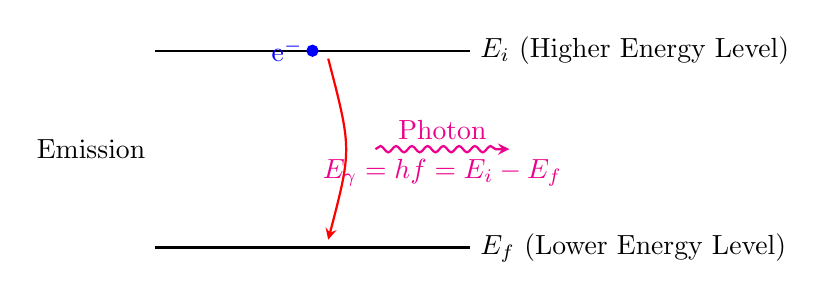
\begin{tikzpicture}[>=stealth]
    % Energy levels
    \draw[thick] (-2, 2.5) -- (2, 2.5) node[right] {$E_i$ (Higher Energy Level)};
    \draw[thick] (-2, 0) -- (2, 0) node[right] {$E_f$ (Lower Energy Level)};
    
    % Electron transition
    \filldraw[blue] (0, 2.5) circle (2pt);
    \draw[->, thick, red] (0.2, 2.4) .. controls (0.5, 1.25) .. (0.2, 0.1);
    \node[left, blue] at (0, 2.5) {e$^-$};
    
    % Emitted photon
    \draw[->, thick, magenta, decorate, decoration={snake,amplitude=0.4mm,segment length=2mm,post length=1mm}] (0.8, 1.25) -- (2.5, 1.25);
    \node[above, magenta] at (1.65, 1.25) {Photon};
    \node[below, magenta] at (1.65, 1.25) {$E_{\gamma} = hf = E_i - E_f$};
    
    \node[left] at (-2, 1.25) {Emission};
\end{tikzpicture}
\caption{Diagram of an electron emitting a photon as it transitions to a lower energy level.}
\end{figure}

\subsection*{Key Equations with Examples}

\subsubsection*{Energy of an Electron in a Hydrogen-like Atom}
The energy of an electron in the n-th state of an atom with atomic number Z is given by:
$$E_n = -\frac{13.6 \cdot Z^2}{n^2} \text{ eV}$$
The negative sign indicates that the electron is bound to the nucleus. An energy of 0 eV corresponds to a free, unbound electron (ionization).

\textbf{Example:}
\begin{itemize}
    \item[(a)] Find the energy of an electron in the ground state (n=1) of a hydrogen atom (Z=1).
    $$E_1 = -\frac{13.6 \cdot 1^2}{1^2} = -13.6 \text{ eV}$$
    \item[(b)] Find the energy of an electron in the first excited state (n=2) of a singly ionized helium atom (He$^{+}$, Z=2).
    $$E_2 = -\frac{13.6 \cdot 2^2}{2^2} = -\frac{13.6 \cdot 4}{4} = -13.6 \text{ eV}$$
\end{itemize}

\subsubsection*{Energy of an Emitted/Absorbed Photon}
The energy of the photon ($E_{\text{photon}}$) involved in a transition is the difference between the initial ($E_i$) and final ($E_f$) energy levels of the electron:
$$E_{\text{photon}} = |\Delta E| = |E_f - E_i|$$
This energy is related to the photon's frequency ($f$) and wavelength ($\lambda$) by the Planck-Einstein relation:
$$E_{\text{photon}} = hf = \frac{hc}{\lambda}$$
A useful conversion is $hc \approx 1240$ eV$\cdot$nm.

\textbf{Example:}
An electron in a hydrogen atom falls from the n=3 state to the n=2 state. What is the wavelength of the emitted photon?
\begin{enumerate}
    \item Find the initial and final energies:
    $E_3 = -13.6/3^2 \approx -1.51$ eV\\
    $E_2 = -13.6/2^2 = -3.40$ eV
    \item Calculate the photon energy:
    $E_{\text{photon}} = |E_2 - E_3| = |-3.40 - (-1.51)| = 1.89$ eV
    \item Calculate the wavelength:
    $$\lambda = \frac{hc}{E_{\text{photon}}} = \frac{1240 \text{ eV}\cdot\text{nm}}{1.89 \text{ eV}} \approx 656 \text{ nm}$$
    This corresponds to the red line (H-alpha) in hydrogen's visible spectrum.
\end{enumerate}

\subsubsection*{Conservation Laws in Collisions}
When atoms collide with other particles, \textbf{total energy} and \textbf{total momentum} are conserved. If the atom's internal energy changes (excitation), the collision is \textbf{inelastic}, and kinetic energy is not conserved.

\textbf{Example:}
An electron with 11.0 eV of kinetic energy collides with a hydrogen atom in its ground state (n=1). Can it excite the atom to the n=2 state? If so, what is the electron's remaining kinetic energy?
\begin{enumerate}
    \item Calculate the energy required for the excitation:
    $\Delta E_{1 \to 2} = E_2 - E_1 = (-3.4 \text{ eV}) - (-13.6 \text{ eV}) = 10.2$ eV
    \item Compare the electron's energy to the required energy. Since the electron's initial kinetic energy (11.0 eV) is greater than the required excitation energy (10.2 eV), the excitation is \textbf{possible}.
    \item The remaining kinetic energy of the electron is:
    $K_{\text{final}} = K_{\text{initial}} - \Delta E_{\text{excitation}} = 11.0 \text{ eV} - 10.2 \text{ eV} = 0.8$ eV.
\end{enumerate}

\newpage
\section*{Problem Solutions}
\hrulefill

\subsection*{Problem 1 (SPhO 2023)}
\begin{quote}
A hydrogen atom is initially at rest. An electron in the hydrogen atom makes a transition from the state with $n=3$ to the state with $n=1$. Calculate the recoil speed and recoil energy of the hydrogen during the process. [Mass of hydrogen atom is $1.66\times10^{-27}$ kg]
\end{quote}

\textbf{Solution:}
\begin{enumerate}
    \item \textbf{Calculate the energy of the emitted photon.}
    The energy of the photon ($E_\gamma$) is equal to the energy difference between the n=3 and n=1 states of the hydrogen atom.
    $$E_n = -\frac{13.6 \text{ eV}}{n^2}$$
    $$E_{\gamma} = E_3 - E_1 = \left(-\frac{13.6}{3^2}\right) - \left(-\frac{13.6}{1^2}\right) = 13.6 \left(1 - \frac{1}{9}\right) = 13.6 \times \frac{8}{9} \approx 12.09 \text{ eV}$$
    Convert this energy to Joules:
    $$E_{\gamma} = 12.09 \text{ eV} \times (1.602 \times 10^{-19} \text{ J/eV}) \approx 1.936 \times 10^{-18} \text{ J}$$

    \item \textbf{Apply Conservation of Momentum.}
    The atom is initially at rest, so the initial momentum is zero. To conserve momentum, the atom must recoil with a momentum ($p_{\text{atom}}$) equal in magnitude and opposite in direction to the momentum of the emitted photon ($p_\gamma$).
    $$|p_{\text{atom}}| = |p_{\gamma}|$$
    The momentum of a photon is given by $p_{\gamma} = E_{\gamma} / c$.
    $$p_{\gamma} = \frac{1.936 \times 10^{-18} \text{ J}}{3.0 \times 10^8 \text{ m/s}} \approx 6.453 \times 10^{-27} \text{ kg m/s}$$
    Therefore, $p_{\text{atom}} = 6.453 \times 10^{-27}$ kg m/s.

    \item \textbf{Calculate the Recoil Speed.}
    The recoil speed ($v_{\text{recoil}}$) of the hydrogen atom is its momentum divided by its mass ($m_H$).
    $$v_{\text{recoil}} = \frac{p_{\text{atom}}}{m_H} = \frac{6.453 \times 10^{-27} \text{ kg m/s}}{1.66 \times 10^{-27} \text{ kg}} \approx 3.89 \text{ m/s}$$

    \item \textbf{Calculate the Recoil Energy.}
    The recoil kinetic energy ($E_{\text{recoil}}$) of the atom is:
    $$E_{\text{recoil}} = \frac{1}{2} m_H v_{\text{recoil}}^2 = \frac{p_{\text{atom}}^2}{2m_H}$$
    $$E_{\text{recoil}} = \frac{(6.453 \times 10^{-27})^2}{2 \times (1.66 \times 10^{-27})} \approx 1.25 \times 10^{-26} \text{ J}$$
\end{enumerate}
\textbf{Final Answers:} Recoil Speed: \textbf{3.89 m/s}, Recoil Energy: \textbf{$1.25 \times 10^{-26}$ J}

\hrulefill
\subsection*{Problem 2 (SPhO 2020)}
\begin{quote}
A free electron collides with a hydrogen atom which is in the ground state. After the collision, the hydrogen atom is excited and during the process of de-excitation, two photons are emitted. The wavelength of one of the photons emitted is 656.3 nm. The electron, after the collision, has de Broglie wavelength of 1.915 nm.\\
(a) What is the wavelength of the other photon emitted during the de-excitation?\\
(b) What is the speed of the free electron before collision?
\end{quote}

\textbf{Solution:}
\begin{description}
    \item[(a) Wavelength of the other photon]
    \begin{enumerate}
        \item \textbf{Identify the first transition.} The emission of a photon with $\lambda_1 = 656.3$ nm corresponds to the transition from n=3 to n=2 in the hydrogen atom.
        \item \textbf{Determine the de-excitation path.} Two photons are emitted as the atom de-excites to the ground state ($n=1$). Since one transition is $3 \to 2$, the other must be $2 \to 1$. This implies the collision excited the atom from $n=1$ to $n=3$.
        \item \textbf{Calculate the wavelength of the second photon ($2 \to 1$).}
        $$\Delta E_{2 \to 1} = 13.6 \left(\frac{1}{1^2} - \frac{1}{2^2}\right) = 13.6 \left(\frac{3}{4}\right) = 10.2 \text{ eV}$$
        $$\lambda_2 = \frac{hc}{\Delta E_{2 \to 1}} = \frac{1240 \text{ eV nm}}{10.2 \text{ eV}} \approx 121.6 \text{ nm}$$
    \end{enumerate}
    \item[(b) Speed of the electron before collision]
    \begin{enumerate}
        \item \textbf{Apply Conservation of Energy.} $K_{\text{initial}} = \Delta E_{\text{excitation}} + K_{\text{final}}$. The excitation is from $n=1$ to $n=3$.
        $$\Delta E_{1 \to 3} = 13.6 \left(\frac{1}{1^2} - \frac{1}{3^2}\right) = 13.6 \left(\frac{8}{9}\right) \approx 12.09 \text{ eV}$$
        \item \textbf{Calculate the final kinetic energy of the electron.} From its de Broglie wavelength $\lambda_{dB} = 1.915$ nm:
        $$p = \frac{h}{\lambda_{dB}} = \frac{6.626 \times 10^{-34} \text{ J s}}{1.915 \times 10^{-9} \text{ m}} \approx 3.46 \times 10^{-25} \text{ kg m/s}$$
        $$K_{\text{final}} = \frac{p^2}{2m_e} = \frac{(3.46 \times 10^{-25})^2}{2 \times (9.11 \times 10^{-31})} \approx 6.57 \times 10^{-20} \text{ J} \approx 0.41 \text{ eV}$$
        \item \textbf{Calculate the initial kinetic energy and speed.}
        $$K_{\text{initial}} = 12.09 \text{ eV} + 0.41 \text{ eV} = 12.50 \text{ eV} \approx 2.00 \times 10^{-18} \text{ J}$$
        $$v_{\text{initial}} = \sqrt{\frac{2K_{\text{initial}}}{m_e}} = \sqrt{\frac{2 \times (2.00 \times 10^{-18})}{9.11 \times 10^{-31}}} \approx 2.09 \times 10^6 \text{ m/s}$$
    \end{enumerate}
\end{description}
\textbf{Final Answers:} (a) Wavelength: \textbf{121.6 nm}, (b) Speed: \textbf{$2.09 \times 10^6$ m/s}

\hrulefill
\subsection*{Problem 3 (SPhO 2019)}
\begin{quote}
An electron, travelling at a speed of $2.08 \times 10^{6}$ m/s collides with a stationary hydrogen atom which is in a state in which its orbital angular momentum is $h/\pi$. What are the possible wavelengths of the photons emitted by the hydrogen atom after collision?
\end{quote}

\textbf{Solution:}
\begin{enumerate}
    \item \textbf{Determine the initial state of the hydrogen atom.}
    Angular momentum (L) is quantized: $L = n \frac{h}{2\pi}$. Given $L = \frac{h}{\pi}$:
    $$n \frac{h}{2\pi} = \frac{h}{\pi} \implies n=2$$
    The atom is initially in the first excited state ($n=2$).

    \item \textbf{Calculate the kinetic energy of the incoming electron.}
    $$K_e = \frac{1}{2} m_e v^2 = \frac{1}{2} (9.11 \times 10^{-31} \text{ kg}) (2.08 \times 10^6 \text{ m/s})^2 \approx 1.97 \times 10^{-18} \text{ J} \approx 12.3 \text{ eV}$$

    \item \textbf{Identify possible excitations.}
    The electron's kinetic energy (12.3 eV) is the maximum energy it can transfer. The ionization energy from the $n=2$ state is $E_{\infty} - E_2 = 0 - (-13.6/2^2) = 3.4$ eV. Since $12.3 \text{ eV} > 3.4 \text{ eV}$, the electron has enough energy to excite the atom to \textbf{any} higher level ($n \ge 3$) or ionize it.

    \item \textbf{Determine possible emission wavelengths.}
    Since any excited state $n \ge 3$ is possible, all downward transitions are possible. The principal emissions from excitation to the $n=3$ level are:
    \begin{itemize}
        \item $3 \to 1$: $\Delta E = 12.09$ eV $\implies \lambda = \frac{1240}{12.09} \approx \textbf{102.6 nm}$
        \item $3 \to 2$: $\Delta E = 1.89$ eV $\implies \lambda = \frac{1240}{1.89} \approx \textbf{656.3 nm}$
        \item $2 \to 1$: $\Delta E = 10.2$ eV $\implies \lambda = \frac{1240}{10.2} \approx \textbf{121.6 nm}$ (This photon can be emitted after the $3 \to 2$ transition).
    \end{itemize}
\end{enumerate}
\textbf{Final Answer:} The electron has sufficient energy to excite the atom to any higher level. The most prominent possible wavelengths are \textbf{102.6 nm}, \textbf{121.6 nm}, and \textbf{656.3 nm}.

\hrulefill
\subsection*{Problem 4 (SPhO 2018)}
\begin{quote}
A singly ionized helium (He$^{+}$), with electron in its ground state n=1, is at rest. A neutron of kinetic energy 68.2 eV collides inelastically with it. The neutron is scattered at an angle of 90$^{\circ}$. The singly ionized helium after collision is excited. Find the allowed values of the kinetic energy of the scattered neutron and the kinetic energy of the single ionized helium after collision. [Mass of He$^{+}$ is four times the mass of the neutron, and energy levels in He$^{+}$ are $E_n = -54.4/n^2$ eV.]
\end{quote}

\begin{figure}[h!]
\centering
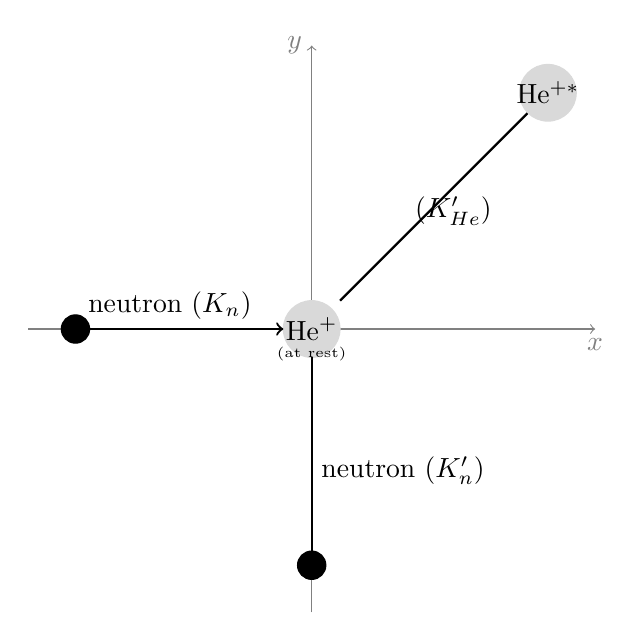
\begin{tikzpicture}[scale=1.2]
    % Axes
    \draw[->, gray] (-3,0) -- (3,0) node[below] {$x$};
    \draw[->, gray] (0,-3) -- (0,3) node[left] {$y$};
    
    % Initial He+ at rest
    \filldraw[gray!30] (0,0) circle (0.3cm);
    \node at (0,0) {He$^{+}$};
    \node[below=0.1cm] at (0,0) {\tiny (at rest)};
    
    % Incident neutron
    \draw[->, thick] (-2.5,0) -- (-0.3,0);
    \filldraw[black] (-2.5,0) circle (0.15cm);
    \node[above] at (-1.5,0) {neutron ($K_n$)};
    
    % Scattered neutron
    \draw[->, thick] (0,-0.3) -- (0,-2.5);
    \filldraw[black] (0,-2.5) circle (0.15cm);
    \node[right] at (0,-1.5) {neutron ($K_n'$)};
    
    % Recoiling He+
    \draw[->, thick] (0.3,0.3) -- (2.5,2.5);
    \filldraw[gray!30] (2.5,2.5) circle (0.3cm);
    \node at (2.5,2.5) {He$^{+*}$};
    \node[below] at (1.5,1.5) {($K_{He}'$)};
\end{tikzpicture}
\caption{Diagram of the neutron-He$^{+}$ collision.}
\end{figure}

\textbf{Solution:} Let $m$ be the mass of the neutron and $K_n = 68.2$ eV. Mass of He$^{+}$ is $M=4m$. Final kinetic energies are $K_n'$ and $K_{He}'$.
\begin{enumerate}
    \item \textbf{Conservation of Momentum:}
    \begin{itemize}
        \item x-dir: $p_{ni} = p'_{He,x} \implies \sqrt{2mK_n} = p'_{He,x}$
        \item y-dir: $0 = -p_{nf} + p'_{He,y} \implies \sqrt{2mK_n'} = p'_{He,y}$
    \end{itemize}
    The total final momentum of the helium ion is $(p'_{He})^2 = (p'_{He,x})^2 + (p'_{He,y})^2 = 2mK_n + 2mK_n'$. Since $K'_{He} = (p'_{He})^2 / (2M) = (2mK_n + 2mK_n') / (8m)$, we get:
    $$4K'_{He} = K_n + K_n'$$

    \item \textbf{Conservation of Energy:} The initial kinetic energy is converted into final kinetic energies plus the excitation energy ($\Delta E$).
    $$K_n = K_n' + K'_{He} + \Delta E$$
    Substitute $K'_{He}$ from the momentum equation:
    $$K_n = K_n' + \frac{K_n + K_n'}{4} + \Delta E \implies 3K_n - 4\Delta E = 5K_n'$$

    \item \textbf{Allowed Excitation Energies:} $\Delta E = E_{n'} - E_1 = 54.4 (1 - 1/n'^2)$ eV. Since $K_n' > 0$, we require $3K_n > 4\Delta E \implies 3(68.2) > 4\Delta E \implies \Delta E < 51.15$ eV.
    \begin{itemize}
        \item n'=2: $\Delta E = 54.4 (1 - 1/4) = 40.8$ eV (Allowed)
        \item n'=3: $\Delta E = 54.4 (1 - 1/9) \approx 48.36$ eV (Allowed)
        \item n'=4: $\Delta E = 54.4 (1 - 1/16) = 51.0$ eV (Allowed)
        \item n'=5: $\Delta E = 54.4 (1 - 1/25) \approx 52.2$ eV (Not allowed)
    \end{itemize}

    \item \textbf{Calculate Final Kinetic Energies for Each Case:}
    \begin{itemize}
        \item \textbf{Case 1 ($n'=2$):} $\Delta E = 40.8$ eV
        $$K_n' = \frac{3(68.2) - 4(40.8)}{5} = \textbf{8.28 eV}$$
        $$K_{He}' = \frac{68.2 + 8.28}{4} = \textbf{19.12 eV}$$
        
        \item \textbf{Case 2 ($n'=3$):} $\Delta E = 48.36$ eV
        $$K_n' = \frac{3(68.2) - 4(48.36)}{5} \approx \textbf{2.23 eV}$$
        $$K_{He}' = \frac{68.2 + 2.23}{4} \approx \textbf{17.61 eV}$$

        \item \textbf{Case 3 ($n'=4$):} $\Delta E = 51.0$ eV
        $$K_n' = \frac{3(68.2) - 4(51.0)}{5} = \textbf{0.12 eV}$$
        $$K_{He}' = \frac{68.2 + 0.12}{4} = \textbf{17.08 eV}$$
    \end{itemize}
\end{enumerate}
\textbf{Final Answer:} The allowed pairs of kinetic energies ($K_n'$, $K_{He}'$) are: \textbf{(8.28 eV, 19.12 eV)}, \textbf{(2.23 eV, 17.61 eV)}, and \textbf{(0.12 eV, 17.08 eV)}.

\end{document}